\chapter{Software Implementation of the Optimizer}\label{ch:implementation}
This Chapter will better analyze the actual implementation of a 3D Optimizer. In particular, it has been developed a self-consistent C++ library that provides all the tools needed to create and optimize 3D graphs that contain \textit{pose} or \textit{point} objects. The main components of the system are basically two:

\begin{enumerate}
    \item The \texttt{Optimizer} itself that runs the Gauss-Newton algorithm to retrieve the best state configuration given the constraints.
    \item The \texttt{Graph}, that contains the actual nodes and edges generated by a suitable front-end or read from file.
\end{enumerate}

While the \texttt{Graph} is just a \textit{container} for nodes and edges, the optimizer has to perform several computations in order to retrieve the linear system $\hessian \dx = -\bvec$ and then solve it. Therefore, underlying the optimizer a linear solver is required to efficiently solve the aforementioned system. 

Once that the front-end populates the graph (or it is loaded from a file), it is fed as input of the optimizer; the general work-flow of a graph optimizer is the following:

\begin{enumerate}
    \item \textbf{Linearization}: for each edge it is computed the error with respect to the current system state and then the relative Jacobian. The output of this phase is the contribution of the edge to the Hessian matrix and the right-hand-side vector.
    \item \textbf{Permutation}: once that the Hessian $\hessian$ is built, it is necessary to compute a proper permutation to reduce Cholesky factorization's fill-in and apply it to Hessian and the right-hand-side vector.
    \item \textbf{Linear Solver}: now it is possible to compute the actual Cholesky factorization $\L$ and retrieve $\dx$ via \textit{Forward/Backward Substitution}.
    \item \textbf{Update}: finally, once that $\dx$ is computed, it is possible to apply it to the current system state -  i.e. to all the graph's \texttt{Vertex}.
\end{enumerate}

It is good to notice that our system is almost completely self-contained: the only external libraries employed are \textit{Eigen} \cite{eigen} - to efficiently manage small matrices  - and \textit{SuiteSparse} \cite{suitesparse} - in order to compute the right permutation of the Hessian. Furthermore, the library has been developed with simplicity and keeping a minimalistic approach, in order to be comprehensible also by researchers that are not expert in this field. Just for comparison, the entire library has less than $6$ thousand lines of code; other state-of-the-art systems are deployed in huge libraries with thousands of lines of code - e.g. \texttt{g2o} \cite{kummerle2011g} is over $40$ thousands lines of code, \texttt{Ceres} \cite{ceres-solver} is over $90$ thousands lines of code and \texttt{gtsam} \cite{dellaert2012gtsam} over $300$ thousands lines of code.

\section{Graph}\label{sec:graph_implementation}
The \texttt{Graph} is basically constituted by a collection of edges and nodes. The nodes can be either of type \textit{pose} or \textit{point} - represented respectively by the objects \texttt{VertexSE3} and \texttt{VertexR3}. Each vertex is represented by

\begin{itemize}
    \item Its \textbf{estimate}, which can be a 3D isometry or a 3D position - namely a \texttt{Pose3D} or a \texttt{Point3D};
    \item A unique \textbf{index} that is used to recognize the vertex;
    \item A boolean variable that indicates whether the node is \textbf{fixed} or not. A fixed Vertex must not be involved in the optimization process. It is good to notice that at least one fixed vertex must exists in the graph, otherwise the optimization problem is undefined.
\end{itemize}

Analogously, the edge are of type \textit{pose-pose} or \textit{pose-point} - represented respectively by the objects \texttt{EdgeSE3} and \texttt{EdgeSE3\_R3}. The edge have several fields, namely:

\begin{itemize}
    \item The actual \textbf{measurement} that can be either a \texttt{Pose3D} or a \texttt{Point3D};
    \item The \textbf{data association} that consists in a pair of \texttt{Vertex} which represents the nodes involved in the edge;
    \item The \textbf{information matrix} related to the measurement - namely a \texttt{Matrix6} or a \texttt{Matrix3}.
\end{itemize}

Once that the front-end populates the graph, it is fed into the \texttt{Optimizer} to perform MAP estimation of the best state configuration given the constraints.
\section{The Optimizer}\label{sec:optimizer}
The \texttt{Optimizer} represents systems' heart: it takes as input the graph, retrieves the linear system $\hessian \dx = -\bvec$, solves for $\dx$ and finally updates the graph. In the following Subsections the core elements of the \texttt{Optimizer} will be better investigated.

\subsection{Linearization and Hessian Composition}\label{subsec:linearize}
One of \texttt{Optimizer}'s tasks is to compute the contribution that each edge brings to both the Hessian matrix $\hessian$ and the right-hand-side vector $\bvec$. Those contribution are retrieved during the \textit{linearization} of the graph. 

Each edge of the graph is analyzed, whether it is a \texttt{EdgeSE3} or a  \texttt{EdgeSE3\_R3}. For each measurement the block matrices $\hessian_{ii}$, $\hessian_{ij}$, $\hessian_{ji}$ and $\hessian_{jj}$ are computed as
\begin{empheq}[box={\mybluebox[3pt]}]{equation}
    \label{eq:j_omega_j}
    \begin{matrix}
        \hessian_{ii} = \jacob_i^T \Omega_k \jacob_i & \hessian_{jj} = \jacob_j^T \Omega_k \jacob_j \\
        \hessian_{ij} = \jacob_i^T \Omega_k \jacob_j & \hessian_{ji} = \jacob_j^T \Omega_k \jacob_i
    \end{matrix}
\end{empheq}
\noindent while the right-hand-side contributions are computed as 

\begin{empheq}[box={\mybluebox[3pt]}]{equation}
    \label{eq:j_omega_e}
    \bvec_i = \jacob_i^T \Omega_k \error_k \qquad \bvec_j = \jacob_j^T \Omega_k \error_k
\end{empheq}

The subscript indexes $\langle i, j \rangle$ are the node unique indexes in the current edge's data-association. The tuple $\langle i, j \rangle$ indicates the position of each block in the full Hessian $\hessian$ (and in the full right-hand-side vector $\bvec$).

The Jacobians $\jacob_i$ and $\jacob_j$ are using Equations \ref{eq:jac_i_se3} and \ref{eq:jac_j_se3} for pose constraints, while for point ones Equations \ref{eq:jac_r_se3r3} and \ref{eq:jac_l_se3r3}. Clearly, as reported in Section \ref{sec:se3_objects}, the information matrix of each \texttt{EdgeSE3} is adapted through the Unscented Transform before starting the optimization process - and \textit{not} at each iteration.

\subsection{Sparse Linear Solver}\label{subsec:sparse_linear_solver}
The linear solver employed is based on Cholesky decomposition of the Hessian - i.e. Subsection \ref{subsec:cholesky_dec_general}. Clearly, the first thing needed in order to efficiently solve a sparse linear system is a proper matrix data-structure.

In this work, sparse matrices are represented through the \texttt{SparseBlockMatrix} object, which uses as storage method the \textit{List of Lists} (LIL) approach. It is possible to select between \textit{fixed-size} blocks - i.e. in pose graph optimization - and \textit{dynamic} blocks - i.e. in pose-landmark graph optimization. In the former case it is possible to take advantage of CPU cache while doing matrix operations and, thus, boosting the computation; using dynamic blocks matrix operations are slower but it adds flexibility to the system. \texttt{SparseBlockMatrix} main feature is the fact that object's memory - used to actually \textit{store} the blocks - can be isolated from the objects itself. Therefore, the actual matrix is just a \textit{view} of those blocks, intended as a LIL of pointers to those memory blocks. This formulation allows to manipulate the \texttt{SparseBlockMatrix} \textbf{without touching the memory}, just rearranging matrix's \textit{view}. The object \texttt{DenseBlockVector} is designed  on the basis of this and it used to store dense vectors like the right-hand-side vector $\bvec$ and the update vector $\dx$.

Before computing the Cholesky factorization, Hessian's non-zero pattern is analyzed through the SuiteSparse library in order to retrieve a suitable ordering that reduces Cholesky's fill-in. The user can choose between different algorithms - i.e. AMD, COLAMD, CHOLMOD - or let the system retrieve the best one.

Once the permutation is found, \texttt{SparseBlockMatrix}'s view of matrix $\hessian$ is rearranged based on the permutation, together with the \texttt{DenseBlockVector} $\bvec$. Now it is possible to compute the Cholesky factorization and retrieve the matrices $\L$ and $\L^T$. Finally, through Forward-Backward Substitution, the update vector $\dx$ is found.

It is good to notice that before solving the linear system, it is necessary to remove fixed vertexes' contribution from the system. Supposing that node $f$ is fixed, then it is necessary to remove the $f$-th row and column from the Hessian, together with the $f$-th block of the $\bvec$. Therefore the system we solve has dimension $n - F$, where $F$ represents the number of fixed vertexes.

\subsection{Graph Update}\label{subsec:update}
Once that the \texttt{DenseBlockVector} $\dx$ is computed, it is necessary to apply to each node $k$ the relative block $\dx_k$ of the update vector.

The update is applied node by node through the \textit{box-plus} operator described in Equations \ref{eq:boxplus_se3} for $SE(3)$ nodes and the Euclidean minus for $\mathbb{R}^3$ ones. Clearly, fixed nodes will remain unchanged. 

\section{Bottlenecks}\label{sec:bottlenecks}
The system has been designed to deliver real-time performances, therefore, an ad-hoc implementation is required to achieve such result. The system described in the previous Section has two main time-consuming operations, both performed at each iteration:

\begin{enumerate}
    \item Allocation and management of the memory for the Hessian's blocks;
    \item The actual computation of the Hessian's blocks described in Equation \ref{eq:j_omega_j}.
\end{enumerate}

However, the proposed system tackles both the issue, reducing the time required for each iteration to values comparable to state-of-the-art systems.

\subsection{Memory management}\label{subsec:memory_management}
Allocate the memory blocks for the Hessian $\hessian$ is a time-expensive operation. Furthermore, it is required to allocate memory also for its decomposition $\L$ and $\L^T$ and for the dense vector $\bvec$, $\dx$ and $\mathbf{y}$. Moreover, copying memory - for example to create a permutation of a matrix -  is another time and resource consuming operation. 

The memory copy has been addressed through the separation of matrix view and memory in the \texttt{SparseBlockMatrix} object, as mentioned before. In this way it is possible to create multiple views of a matrix that share the same physical memory, avoiding memory copy and, thus, reducing the memory consumption of the system. The same feature is found in the \texttt{DenseBlockVector} object. The physical memory is managed by a separated object called \texttt{MemoryManager}. It is in charge of allocating, delete and copy memory for matrix and vectors.

However, even if we are able to avoid memory copy, it is necessary to allocate the matrices and vectors at each iteration. Once again, this process is avoided through a clever solution: once the graph is built, it is possible to exploit its structure to evaluate the non-zero pattern of the Hessian $\hessian$. The reader might notice that the non-zero pattern will remain unchanged for the entire optimization process, while the \textit{numeric values} of the block will change at each iteration. Moreover, all the \texttt{DenseBlockVector}s will have a fixed dimension equal to the number of active vertexes $n - F$. Therefore, it is possible to allocate all the memory required to store Hessian's and vectors' block \textbf{only once} before starting the optimization process.

Once that we have the Hessian's non-zero pattern, it is possible to compute both the permutation and the \textit{Cholesky symbolic decomposition}, that retrieves the non-zero pattern of matrix $\L$ (and thus also $\L^T$). In this way, during the optimization steps there is \textbf{no memory allocation or copy}, speeding up the entire system.

\subsection{Hessian blocks computation}\label{subsec:j_omega_j}
Using the \textit{Eigen} library to perform matrix operations, it is possible to appreciate a bottleneck in the computation of the product $\hessian_{ij} = \jacob_i^T \Omega_k \jacob_j$ - and all the other blocks $\hessian_{ii}$, $\hessian_{jj}$ and $\hessian_{ji}$. The slowing down is particularly emphasized for $(6\times6)$ \textit{static} or \textit{dynamic} blocks.

However, for \textit{pose-pose} constraints, given the product $\mathbf{A} = \jacob_i^T \Omega_k \jacob_i$, the following relations hold:

\begin{align*}
    \hessian_{ii} &= \mathbf{A} \quad\qquad
    \hessian_{jj} = \mathbf{A} \\
    \hessian_{ij} &= -\mathbf{A} \:\,\qquad
    \hessian_{ji} = -\mathbf{A}
\end{align*}

\noindent In this way the computation is performed just one time, thus there is a $75\%$ boost in terms of speed. Furthermore, since $\mathbf{A}$ is a symmetric matrix, it is possible to compute just the upper triangular part and then replicate it in the lower triangular, reducing even more the computational time.

\section{Performance Results}\label{sec:performance_results}
The library developed has been tested on different synthetic datasets both in \textit{pose-graph} and \textit{pose-landmark} scenarios. All the test have been performed on a Lenovo ThinkPad W540 laptop equipped with:

\begin{itemize}
    \item CPU: Intel(R) Core(TM) i7-4700MQ CPU @ 2.40GHz
    \item RAM: $2 \times 4$GB $+$ $2\times8$GB SODIMM DDR3 - total 24GB
    \item Disk: SanDisk(R) Ultra II(TM) 240GB Solid State Drive
    \item OS: Ubuntu 16.04 LTS
\end{itemize}

Since the works focuses on \textit{pose-graph} optimization, the results will be mostly related to this kind of problem. In this case the blocks composing the Hessian have fixed size - i.e. $(6\times6)$ - and, therefore, it is possible to employ a \texttt{SparseBlockMatrix} with static fix-sized blocks. 

The experiments proposed are obtained using three different datasets that have an increasing number of edges:

\begin{enumerate}
    \item The open-loop graph created by ProSLAM\_stud from the \textit{Kitti\_00} run (further information in Chapter \ref{ch:cases}), with 752 nodes and 903 edges (easy);
    \item A synthetic sphere with 2500 vertexes and 9799 edges (medium);
    \item A synthetic dataset wit 2001 poses and 24422 edges (hard).
\end{enumerate}

Figure \ref{fig:step_time} shows the step-time's evolution of both systems during the optimization of the three datasets. Furthermore, in Table \ref{tab:total_optimization_time} are reported the total optimization time employed by both systems to execute 10 steps.

\begin{figure}[!hbt]
    \centering
    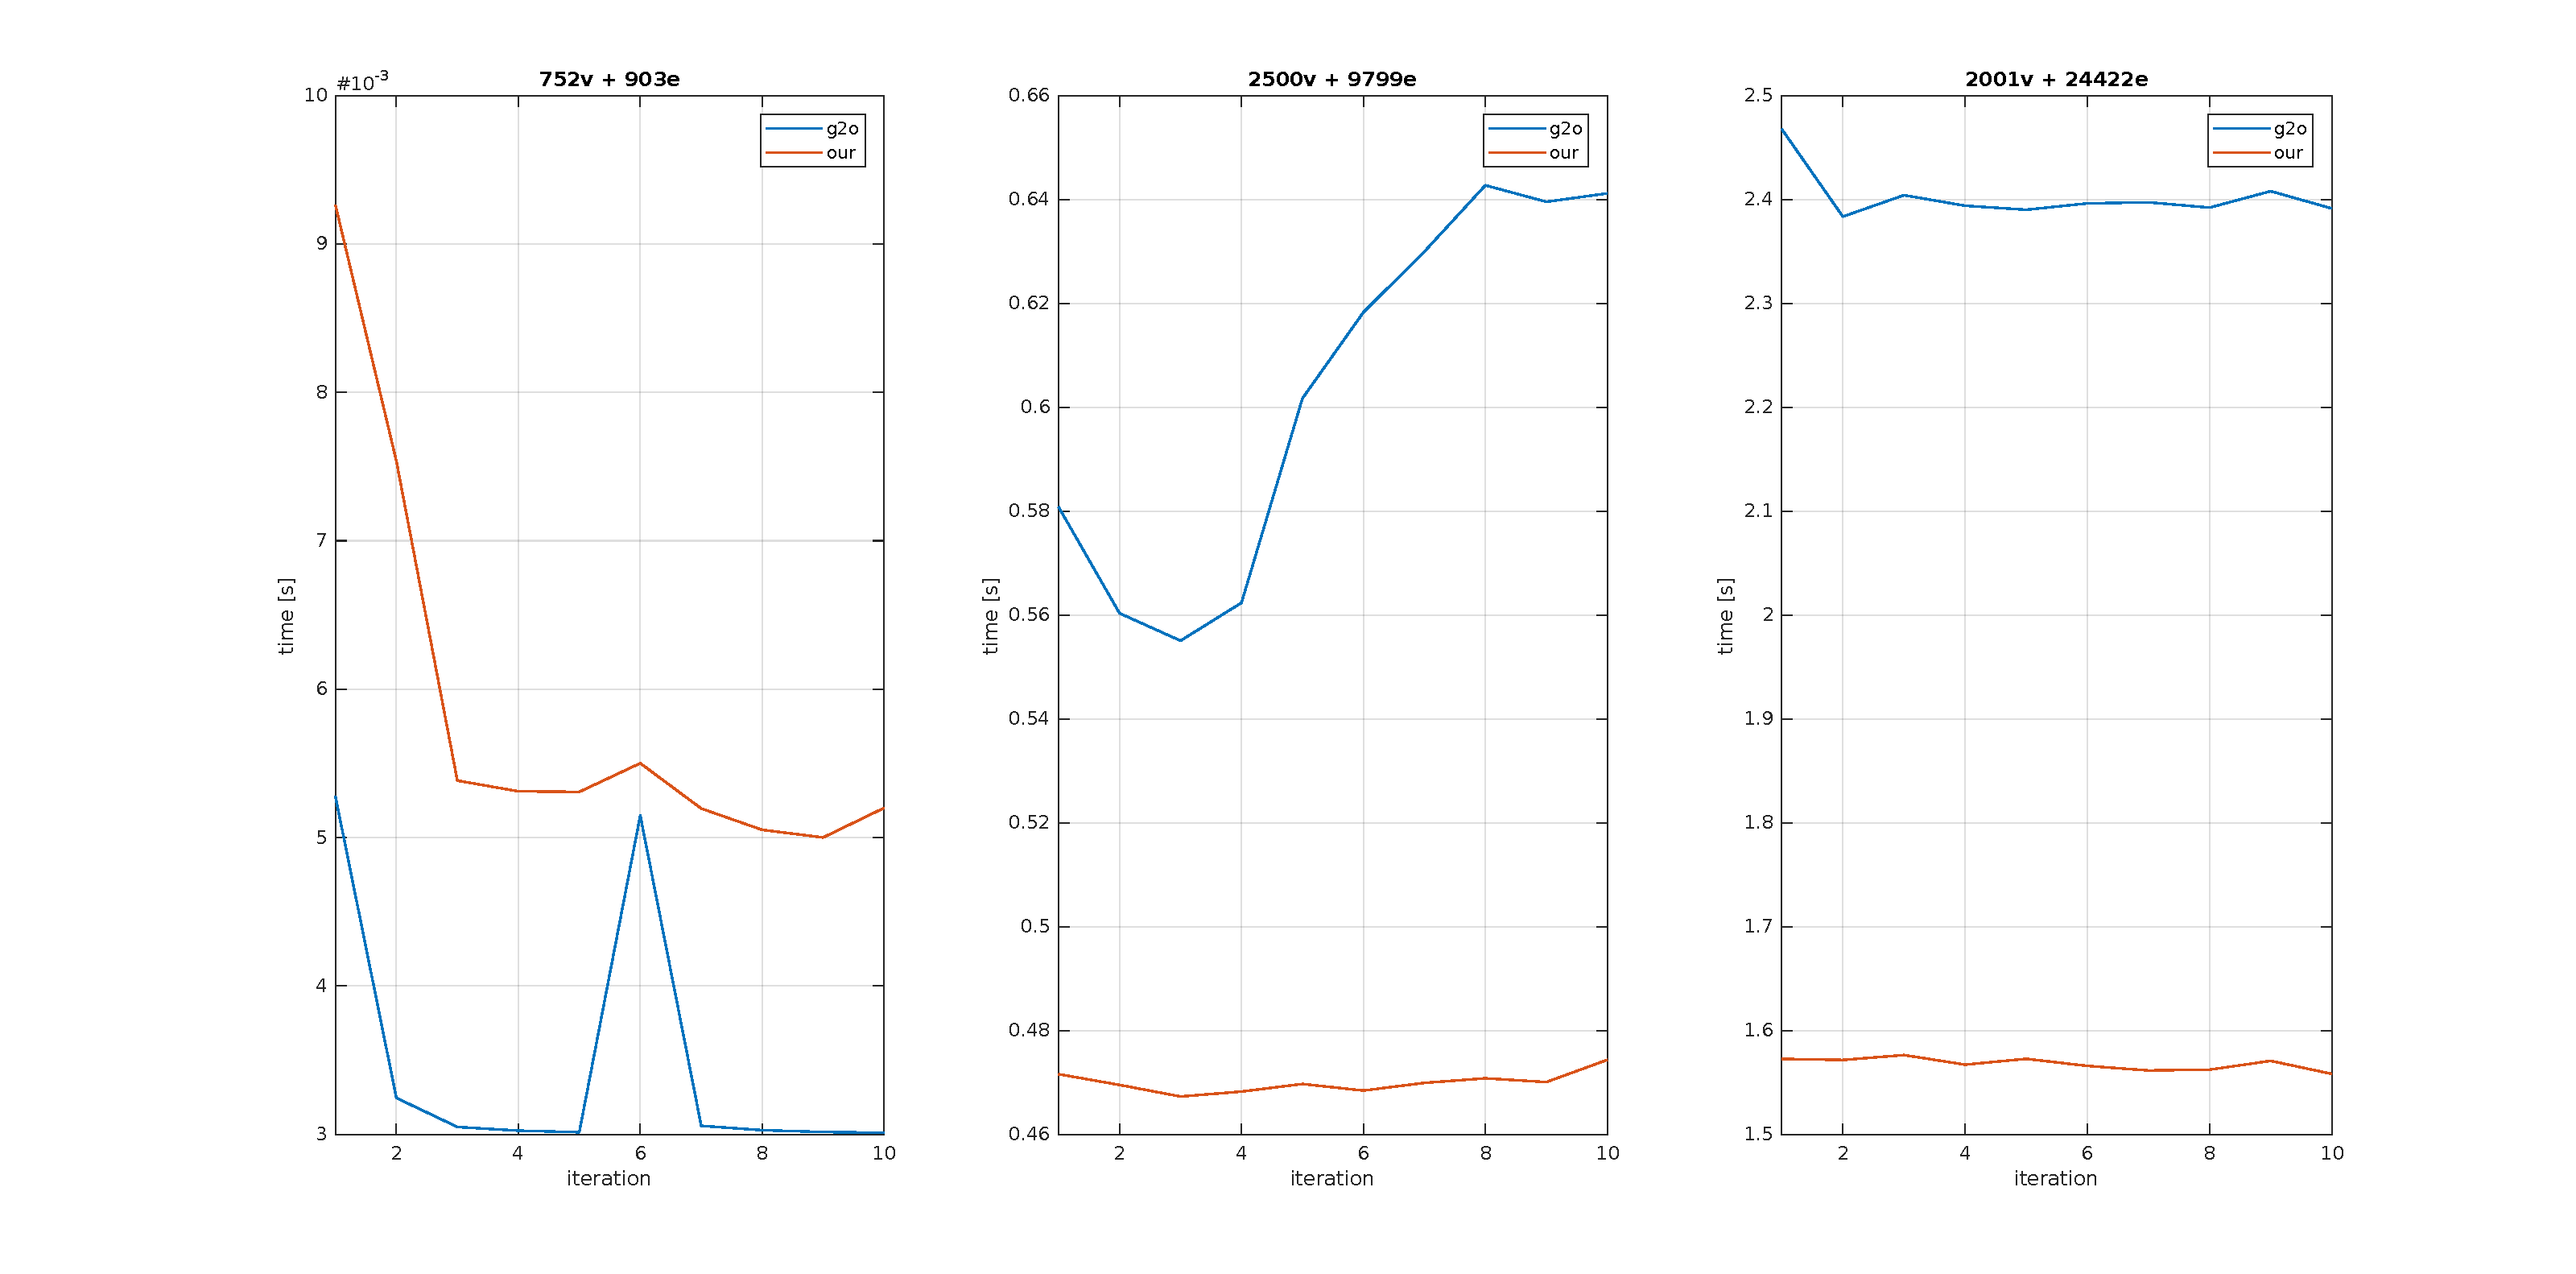
\includegraphics[width=\textwidth]{figures/05_implementation/step_time.pdf}
%    \resizebox{0.7\textwidth}{!}{\input{figures/05_implementation/step_time.pdf}}
    \caption{\textbf{Pose Graph Optimization Step Time Comparison.} Comparison between \texttt{g2o} - in blue - and \textit{our system} - in orange - of the time required to execute an optimization step. Despite the minimalistic implementation, our approach is significantly faster than \texttt{g2o}; the gap increases with the number of edges, indicating a slightly better scalability of the proposed system with respect to \texttt{g2o}.} 
    \label{fig:step_time}
\end{figure}

The reader might notice how well our systems behaves, delivering performances that are better or at least comparable with the one obtained through a state-of-the-art complex system like \texttt{g2o}. Furthermore, the results show that an increased number of edges corresponds to a bigger gap between our approach and \texttt{g2o}, indicating that our implementation is very efficient and slightly more scalable.

\begin{table}[!hbt]
    \centering
    \begin{tabular}{ l l l l }
        \toprule 
        \multicolumn{4}{ c }{\textbf{Total Optimization Time}} \\ \hline
        System & \textit{easy} $[s]$ & \textit{medium} $[s]$ & \textit{hard} $[s]$ \\
        \midrule
        \texttt{g2o} & 0.0349 & 6.0319 & 24.0242  \\ 
        our & 0.0588 & 4.7000 & 15.6795 \\ \hline
    \end{tabular}
    \caption{\textbf{Pose Graph Optimization Total Time Comparison.} In this table are reported the total optimization time required by the two systems to complete 10 iterations. The reader might notice that in graphs with more edges, our approach performs better than \texttt{g2o}.}
    \label{tab:total_optimization_time}
\end{table}

For pose-landmark graphs, our systems struggles to obtain the same results seen in pose-graph optimization. This is mainly due to use of a \texttt{SparseBlockMatrix} with dynamic blocks, that makes our implementation slower than its competitor \texttt{g2o}, as it is reported in Figure \ref{fig:step_time_BA} and Table \ref{tab:total_optimization_time_BA}.

\begin{figure}[!hbt]
    \centering
    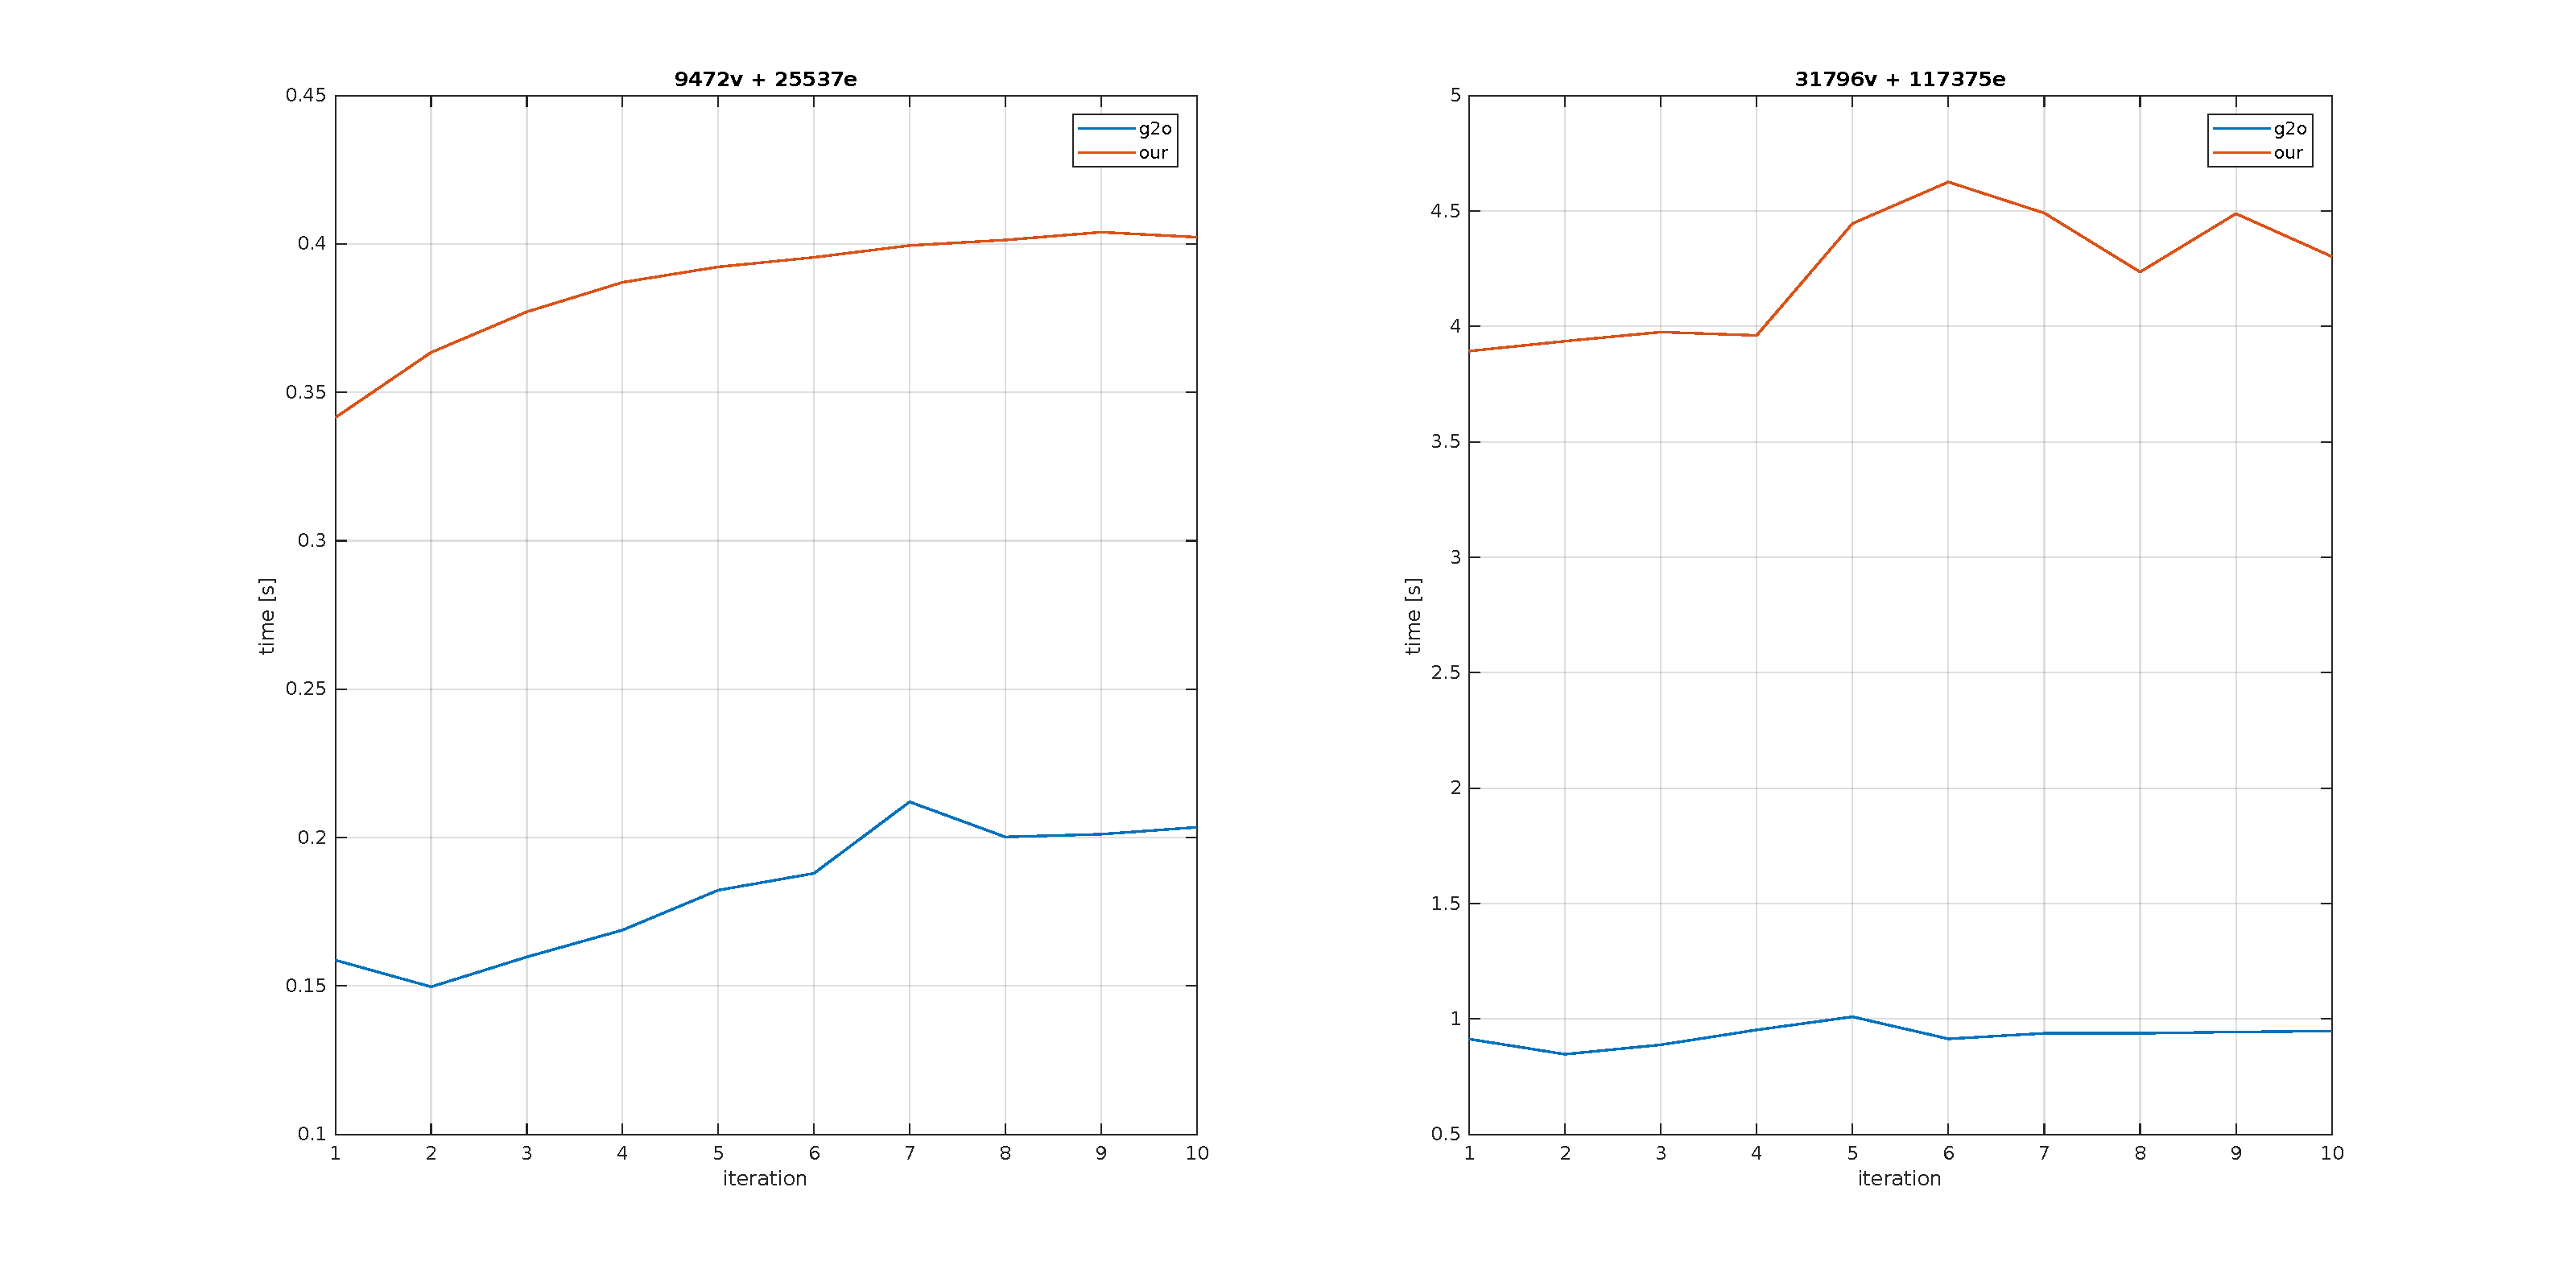
\includegraphics[width=\textwidth]{figures/05_implementation/step_time_BA.pdf}
    \caption{\textbf{BA Optimization Step Time Comparison.} Comparison between \texttt{g2o} - in blue - and \textit{our system} - in orange - of the time required to execute an optimization step. In this case \texttt{g2o} leads always the comparison.} 
    \label{fig:step_time_BA}
\end{figure}

The results are obtained running the two systems on two datasets that have an increasing number of nodes and edges. In particular:

\begin{enumerate}
    \item A synthetic dataset with 9472 vertexes (1001 \texttt{SE3} + 8471 \texttt{R3}) and 25537 edges (6013 \texttt{SE3} + 19524 \texttt{SE3\_R3}) - called \textit{small};
    \item A bigger synthetic dataset that has 31796 vertexes (2001 \texttt{SE3} + 29795 \texttt{R3}) and 117375 edges (25327 \texttt{SE3} + 92048 \texttt{SE3\_R3}) - called \textit{big}.
\end{enumerate}

\begin{table}[!hbt]
    \centering
    \begin{tabular}{ l l l }
        \toprule 
        \multicolumn{3}{ c }{\textbf{Total Optimization Time}} \\ \hline
        System & \textit{small} $[s]$ & \textit{big} $[s]$ \\
        \midrule
        \texttt{g2o} & 1.8242 & 9.2920 \\ 
        our & 3.8641 & 42.3554 \\ \hline
    \end{tabular}
    \caption{\textbf{BA Optimization Total Time Comparison.} In this table are reported the total optimization time required by the two systems to complete 10 iterations. The reader might notice an inverted trend with respect to pure pose-graph optimization, with our system struggling when the number of edges increases.}
    \label{tab:total_optimization_time_BA}
\end{table}

\noindent One possible solution to this bad trend can be the use of static blocks also for BA problems, solving the linear system $\hessian \dx = -\bvec$ using the \textit{Schur Complement}.